% This work is licensed under the Creative Commons Attribution-NonCommercial 4.0 International License.
% To view a copy of this license, visit http://creativecommons.org/licenses/by-nc/4.0/
% or send a letter to Creative Commons, PO Box 1866, Mountain View, CA 94042, USA.

% !TEX TS-program = xelatex

\documentclass[../Main/chem532-notes.tex]{subfiles}
\begin{document}

\chapter{Electronic wave functions}

\section{Spin}
So far we have neglected to account for spin.
To introduce spin, we consider a set of spin operators $\hat{s}_x, \hat{s}_y, \hat{s}_z$, analogous to angular momentum operators.\mnote{We use lower case $s$ for spin operators that act only on one particle. This notation will help us distinguish from the spin operators for a collection of electrons.}
The spin operators satisfy the following commutation relationship
\begin{equation}
[\hat{s}_{j},\hat{s}_{k}] = \hat{s}_{j}\hat{s}_{k} - \hat{s}_{k}\hat{s}_{j}= i \hbar \varepsilon_{jkl} \hat{s}_{l} \quad \text{ with } j,k,l \in \{x,y,z\},
\end{equation}
where $\varepsilon_{jkl}$ is the Levi-Civita symbol defined as
\begin{equation}
\varepsilon_{jkl} = \begin{cases}
+1 & \text{if $(j,k,l)$ is an even permutation of $(x,y,z)$} \\
-1 & \text{if $(j,k,l)$ is an odd permutation of $(x,y,z)$} \\
0 & \text{otherwise}.
\end{cases}
\end{equation}

The total spin operator $\hat{\vec{s}}$ is a vector operator with components
\begin{equation}
\hat{\vec{s}} = (\hat{s}_x, \hat{s}_y, \hat{s}_z).
\end{equation}
We also define the angular momentum squared operator ($\hat{s}^2$) as
\begin{equation}
\hat{s}^2 = \hat{\vec{s}} \cdot \hat{\vec{s}} = \hat{s}_x^2 + \hat{s}_y^2 + \hat{s}_z^2.
\end{equation}
Since the $\hat{s}^2$ commutes with all vector components of $\hat{\vec{s}}$
\begin{equation}
[\hat{s}^2,\hat{s}_j] = 0 \quad \text{ with } j \in \{x,y,z\},
\end{equation}
we can pick one component, say the $z$ axis and introduce a basis of spin functions $\ket{s,m_s}$ that are simultaneous eigenfunctions of $\hat{s}^2$ and $\hat{s}_z$. Note that for a given value of $s$, $m_s$ can take values $s, s -1, s-2, \ldots, -s$.
The spin eigenfunctions satisfy:
\begin{align}
\hat{s}^2 \ket{s,m_s} &= \hbar^2 s(s+1) \ket{s,m_s}, \\
\hat{s}_z \ket{s,m_s} &= \hbar m_s \ket{s,m_s}.
\end{align}

In the case of electrons we have that $s = \frac{1}{2}$, and so we label the two spin functions as $\alpha$ and $\beta$\mnote{Other notations are common. For example $\ket{0}$ and $\ket{1}$ is commonly used in quantum computing and $\ket{\uparrow}$ and $\ket{\downarrow}$ in physics.}
\begin{align}
\ket{\alpha} &= \ket{\frac{1}{2},\frac{1}{2}}, \\
\ket{\beta} &= \ket{\frac{1}{2},-\frac{1}{2}}.
\end{align}

These functions are normalized and orthogonal:
\begin{align}
\braket{\alpha | \alpha} &= \braket{\beta | \beta} = 1, \\
\braket{\alpha | \beta} &= 0. \label{eq:spin_orthogonality}
\end{align}
At times, we might write these functions as
\begin{align}
\alpha(\omega) &= \braket{\omega|\alpha} \\
\beta(\omega) &= \braket{\omega|\beta},
\end{align}
where $\omega$ is a fictitious spin variable. This allow us to treat $\alpha(\omega)$ and $\beta(\omega)$ as traditional wave functions. For example, the orthogonality condition [Eq.~\eqref{eq:spin_orthogonality}] may be written as
\begin{equation}
\braket{\alpha | \beta} = \int d\omega \, \alpha^*(\omega) \beta(\omega)  = 0.
\end{equation}

When talking about spin it is also convenient to introduce the raising ($\hat{s}_{+}$) and lowering ($\hat{s}_{-}$) spin operators.
These are defined as:
\begin{align}
\hat{s}_{+} & = \hat{s}_{x} + i \hat{s}_{y} \\
\hat{s}_{-} & = \hat{s}_{x} - i \hat{s}_{y}  
\end{align}
In the case of $s = \frac{1}{2}$ particles, the action of $\hat{s}_{+}$ and $\hat{s}_{-}$ on the spin eigenfunctions is
\begin{align}
\hat{s}_{+} \ket{\alpha} &= 0, \\
\hat{s}_{+} \ket{\beta} &= \ket{\alpha} \quad (m_s: -\frac{1}{2} \rightarrow \frac{1}{2}),\\
\hat{s}_{-} \ket{\alpha} &= \ket{\beta} \quad (m_s: \frac{1}{2} \rightarrow -\frac{1}{2}),\\
\hat{s}_{-} \ket{\beta} &= 0.
\end{align}
These operator raise or lower the value of $m_s$ or return zero if an eigenfunction with higher (lower) value of $m_s$ does not exist.
The $\hat{s}^2$ operator may be represented using the raising and lowering operators as
\begin{equation}
\hat{s}^2 = \hat{s}_{+}\hat{s}_{-} + \hat{s}^{2}_{z} - \hat{s}_{z}.
\end{equation}

It is also convenient to introduce many-electron generalizations of the spin operators.
For a system of $N$ electrons, we define total spin operators as the sum of operators action on each particle.
\begin{align}
\hat{S}^2 &= \sum_i^N \hat{s}^{2}(i), \\
\hat{S}_z &= \sum_i^N \hat{s}_{z}(i), \\
\hat{S}_+ &= \sum_i^N \hat{s}_{+}(i), \\
\hat{S}_- &= \sum_i^N \hat{s}_{-}(i),
\end{align}
where $\hat{s}^{2}(i)$ means that an operator $\hat{s}^{2}$ acts only on electron $i$.


\section{Spin orbitals}
Let us introduce some important nomenclature.
Functions that describe electrons in real space are called \textbf{spatial orbitals} and we will indicate them with the Greek symbol phi, $\phi_i(\vec{r})$.
In general the set $\{ \phi_i(\vec{r}) \}$ is infinite, complete, and may be orthonormalized.\mnote{A set of functions $\{ \phi_i(\vec{r}) \}$  is called \textbf{orthonormal} if any two functions satisfy $\int d\vec{r} \, \phi_i^*(\vec{r}) \phi_j(\vec{r})  = \delta_{ij}$.}
If the functions $\phi_i(\vec{r})$ are normalized then the quantity $|\phi_i(\vec{r})|^2 d\vec{r}$ is the probability of finding the electron in the volume element $d\vec{r}$.
The completeness condition implies that we can expand any function $f(\vec{r})$ using the set $\{ \phi_i(\vec{r}) \}$
\begin{equation}
f(\vec{r}) = \sum_{i}^{\infty} a_i \phi_i(\vec{r}).
\end{equation}
In practice, we use finite sets, so that $\dim \{ \phi_i(\vec{r}) \} = K < \infty$.

\textbf{Spin orbitals} are the product of a spatial orbital and a spin function:\mnote{We will abbreviate the spatial and spin coordinates with the symbol $x \equiv (\vec{r},\omega)$.}
\begin{equation}
\psi_{i,\sigma} (x) = \psi_{i,\sigma} (\vec{r},\omega) = \phi_i(\vec{r}) \sigma(\omega),
\end{equation}
where $\sigma(\omega) \in \{\alpha(\omega),\beta(\omega)\}$ indicates a generic spin function.
For a basis of spatial orbitals with dimension $K$ we can collect the indices $(i,\sigma)$ in one integer and define $2K$ spin orbitals:
\begin{align}
\psi_{2i - 1}(x) &= \phi_i(\vec{r}) \alpha(\omega), \\
\psi_{2i}(x) &= \phi_i(\vec{r}) \beta(\omega).
\end{align}
Note that if the spatial orbitals are orthonormal, then the spin orbital basis is also orthonormal:
\begin{equation}
\int d\vec{r} \, \psi_i^*(\vec{r}) \psi_j(\vec{r})  = \delta_{ij}.
\end{equation}


\section{$N$-electron wave functions}
How can we build a wave function for $N$ electrons $\Phi(x_1,x_2,\ldots,x_N)$ from a basis of spin orbitals? Pauli's principle requires that $\Phi$ is antisymmetric with respect to odd permutations of the coordinates (spatial and spin) of any two electrons $i$ and $j$:
\begin{equation}
\Phi(\ldots,x_i,\ldots,x_j,\ldots,x_N) = - \Phi(\ldots,x_j,\ldots,x_i,\ldots,x_N).
\end{equation}
Particles whose wave functions satisfies this condition are called \textbf{fermions}.

\begin{example}[Wave function for two electrons]
Consider a system of two electrons. The wave function is $\Phi(x_1,x_2)$ and the antisymmetry requirement is
\begin{equation}
 \Phi(x_2,x_1) = - \Phi(x_1,x_2).
\end{equation}
Now let us assume that we are given a complete spin orbital basis $\{ \psi_{i}(x) \}$.
We can think of $\Phi(x_1,x_2)$ with $x_2$ held constant as a function only of the variable $x_1$.
Therefore, we may expand $\Phi(x_1,x_2)$ using the spin orbital basis as:
\begin{equation}\label{eq:two_electron_wfn_expansion1}
\Phi(x_1,x_2) = \sum_{i}^{\infty} a_i(x_2) \psi_i(x_1),
\end{equation}
notice, however, that the expansions coefficients $a_i(x_2)$ will depend on the value of $x_2$, in other words, $a_i$ is a function of $x_2$.
We can now expand $a_i(x_2)$ using the same spin orbital basis:
\begin{equation}\label{eq:two_electron_wfn_expansion2}
a_i(x_2) = \sum_{j}^{\infty} a_{ij} \psi_j(x_2),
\end{equation}
and introduced the quantity $a_{ij}$, which carries both the indices for the $x_1$ and $x_2$ expansions.
Combining Eqs.~\eqref{eq:two_electron_wfn_expansion1}--\eqref{eq:two_electron_wfn_expansion2} we obtain:
\begin{equation}
\Phi(x_1,x_2) = \sum_{ij}^{\infty} a_{ij} \psi_i(x_1) \psi_j(x_2).
\end{equation}
This functions may satisfy the antisymmetry condition if:
\begin{equation}
\sum_{ij}^{\infty} a_{ij} \psi_i(x_1) \psi_j(x_2) = -\sum_{ij}^{\infty} a_{ij} \psi_i(x_2) \psi_j(x_1).
\end{equation}
To find out the implication of this condition onto the coefficients $a_{ij}$, first perform the index interchange $i \leftrightarrow j$ on the left hand side:
\begin{equation}
\sum_{ij}^{\infty} a_{ij} \psi_i(x_1) \psi_j(x_2) = -\sum_{ij}^{\infty} a_{ji} \psi_j(x_2) \psi_i(x_1),
\end{equation}
and the collect terms that multiply the factor $\psi_i(x_1) \psi_j(x_2)$ to obtain the condition:
\begin{equation}
\label{eq:two_electron_wfn_expansion4}
\sum_{ij}^{\infty} (a_{ij} + a_{ji}) \psi_i(x_1) \psi_j(x_2) = 0.
\end{equation}
Equation~\eqref{eq:two_electron_wfn_expansion4} must hold for any value of $\psi_i(x_1) \psi_j(x_2)$, and this is possible only if
\begin{equation} \label{eq:two_electron_wfn_expansion3}
a_{ij} + a_{ji} = 0.
\end{equation}
This conditions may also be written as 
\begin{equation}
a_{ij} = - a_{ji}.
\end{equation}
As a consequence, the diagonal elements of $a_{ij}$, $a_{ii}$, are zero.\mnote{To see this set $j = i$. Then $a_{ii} + a_{ii} = 2 a_{ii} = 0$, so that $a_{ii} = 0$.}
Eq.~\eqref{eq:two_electron_wfn_expansion3} shows that the when we expand an antisymmetric wave function using a single-particle basis, the antisymmetry condition is reflected in the properties of the coefficients $a_{ij}$.\mnote{The quantity $a_{ij}$ is a skew-symmetric or antisymmetric matrix. For $N$ electrons, the expansion coefficient will be an antisymmetric \textbf{tensor} with $N$ indices, that is $a_{i_1 i_2 i_3 \cdots i_N}$.}


Using Eq.~\eqref{eq:two_electron_wfn_expansion3} we may write the two-electron wave function as:
\begin{equation}
\begin{split}
\Phi(x_1,x_2) &= \sum_{i<j}^{\infty} a_{ij} \psi_i(x_1) \psi_j(x_2) + \sum_{i>j}^{\infty} a_{ij} \psi_i(x_1) \psi_j(x_2) \\
&= \sum_{i<j}^{\infty} a_{ij} \psi_i(x_1) \psi_j(x_2) + \sum_{j>i}^{\infty} a_{ji} \psi_j(x_1) \psi_i(x_2) \\
&= \sum_{i<j}^{\infty} a_{ij} \psi_i(x_1) \psi_j(x_2) - \sum_{i<j}^{\infty} a_{ij} \psi_i(x_2) \psi_j(x_1) \\
&= \sum_{i<j}^{\infty} a_{ij} [ \psi_i(x_1) \psi_j(x_2) - \psi_i(x_2) \psi_j(x_1)].
\end{split}
\end{equation}
The quantity $\psi_i(x_1) \psi_j(x_2) - \psi_i(x_2) \psi_j(x_1)$ can also be expressed as the determinant of a matrix since:
\begin{equation}
\det
\begin{bmatrix}
\psi_i(x_1) & \psi_i(x_2) \\
\psi_j(x_1) & \psi_j(x_2) 
\end{bmatrix}
\equiv
\begin{vmatrix}
\psi_i(x_1) & \psi_i(x_2) \\
\psi_j(x_1) & \psi_j(x_2) 
\end{vmatrix}
=
\psi_i(x_1) \psi_j(x_2) - \psi_i(x_2) \psi_j(x_1).
\end{equation}
Hence we discover that $\Phi(x_1,x_2)$ must be a linear combination of determinants:
\begin{equation}
\Phi(x_1,x_2) = \sum_{i<j}^{\infty} a_{ij} 
\begin{vmatrix}
\psi_i(x_1) & \psi_i(x_2) \\
\psi_j(x_1) & \psi_j(x_2)
\end{vmatrix}.
\end{equation}
\end{example}

A convenient way to represent antisymmetric wave functions for $N$ electrons is to expand it into a basis of functions that is automatically antisymmetric with respect to particle permutations. Such functions are known as \textbf{Slater determinants} and are defined as
\begin{equation}
\Phi_{ijk\cdots}(x_1,x_2,\ldots,x_N) = \frac{1}{\sqrt{N!}} 
\begin{vmatrix}
\psi_i(x_1) & \psi_i(x_2) & \cdots & \psi_i(x_N) \\
\psi_j(x_1) & \psi_j(x_2) & \cdots & \psi_j(x_N) \\
\psi_k(x_1) & \psi_k(x_2) & \cdots & \psi_k(x_N) \\
\vdots & \vdots & \vdots & \vdots
\end{vmatrix}.
\end{equation}
Slater determinants automatically satisfy the antisymmetry requirement of fermionic wave functions because the determinant of a matrix changes sign when two columns are swapped. This operation is equivalent to permuting particle indices.
For convenience we will write a Slater determinant, \textbf{including its normalization factor}, with the compact notation
\begin{equation}
\ket{\Phi_{ijk\cdots}} =\ket{
\psi_i \psi_j \psi_k \cdots},
\end{equation}
omitting the labels of the electrons.
The basis of Slater determinants $\{ \ket{
\psi_i \psi_j \psi_k \cdots} \}$ with $i, j, k, \ldots \in \{0, 1, 2, \ldots \}$ is complete.\mnote{This property is inherited from the fact that the one-electron spin orbital basis is complete.}
Therefore, we may expand any electronic wave function using the Slater determinant basis:
\begin{equation}
\ket{\Psi} = \sum_{i<j<k\cdots} C_{ijk\cdots} \ket{
\psi_i \psi_j \psi_k \cdots}.
\end{equation}
This expansion is called a \textbf{full configuration interaction} (FCI) wave function.
The FCI wave function can provide the exact solution to the electronic Schr\"{o}dinger equation.
In practice, we always work with a finite spin orbital basis. Then we say that the FCI wave function provides the exact solution of the Schr\"{o}dinger equation \textbf{within a finite basis}.
For a system with $N$ electrons and a spin orbital basis of dimension $2K$, the number of determinants in the FCI expansion is given by the number of ways to choose a subset of $N$ electrons, disregarding their order, from a set of $2K$ spin orbitals:
\begin{equation}
N_{\rm FCI} = \binom{2K}{N}.
\end{equation}
$N_{\rm FCI}$ grows very quickly with $N$ and $K$ and so the FCI wave function is impractical for more than 16--18 electrons.


\begin{example}[Hartree products vs. Slater determinants]
Let us compare a wave function that is just a product of spin orbitals with a Slater determinant for a two-electrons system.
A Hartree product is simply the product of orbitals:
\begin{equation}
\Phi^{\rm HP}(x_1,x_2) = \psi_i(x_1) \psi_j(x_2).
\end{equation}
The modulus square of $\Phi^{\rm HP}(x_1,x_2)$ shows that the probability distribution of two electrons is just the product of individual orbital probabilities:
\begin{equation}
| \Phi^{\rm HP}(x_1,x_2)|^2 = |\psi_i(x_1)|^2 |\psi_j(x_2)|^2 = P_i(x_1) P_j(x_2).
\end{equation}
A Hartree product represents a state with \textbf{no correlation}.

A Slater determinant:
\begin{equation}
\Phi^{\rm SD}(x_1,x_2) = \frac{1}{\sqrt{2}} [ \psi_i(x_1) \psi_j(x_2) - \psi_i(x_2) \psi_j(x_1)].
\end{equation}
has a probability distribution equal to:
\begin{equation}
\begin{split}
|\Phi^{\rm SD}(x_1,x_2)|^2 = \frac{1}{2} [&
P_i(x_1) P_j(x_2) +  P_j(x_1) P_i(x_2) \\
&-  \psi_i^*(x_1)\psi_j(x_1)  \psi_j^*(x_2) \psi_i(x_2)\\
&- \psi_j^*(x_1)\psi_i(x_1) \psi_j(x_2) \psi_i^*(x_2)  
].
\end{split}
\end{equation}
The first two terms are symmetrized probability distributions for individual orbitals [$P_i(x_1) P_j(x_2) +  P_j(x_1) P_i(x_2)$], while the third and fourth terms couple the position of electron 1 and 2.
If we integrate $|\Phi^{\rm SD}(x_1,x_2)|^2$ over the spin variables $\omega_1$ and $\omega_2$ we can derive a probability distribution that depends only on the positions of the electrons:
\begin{equation}
P(\mathbf{r}_1,\mathbf{r}_2) =
\int d\omega_1 d\omega_2 |\Phi^{\rm SD}(x_1,x_2)|^2.
\end{equation}
We now distinguish two cases.
If electrons have \textit{different} spin then the probability distribution is symmetric but not correlated:
\begin{equation}
P(\mathbf{r}_1,\mathbf{r}_2) = \frac{1}{2} [
P_i(\mathbf{r}_1) P_j(\mathbf{r}_2) +  P_j(\mathbf{r}_1) P_i(\mathbf{r}_2) ].
\end{equation}
If instead the two electrons have different spin, then the cross terms [$\psi_i^*(\mathbf{r}_1)\psi_j(\mathbf{r}_1)  \psi_j^*(\mathbf{r}_2) \psi_i(\mathbf{r}_2)$] survive and introduce correlation in the probability distribution
\begin{equation}
\begin{split}
P(\mathbf{r}_1,\mathbf{r}_2) = \frac{1}{2} [&
P_i(\mathbf{r}_1) P_j(\mathbf{r}_2) +  P_j(\mathbf{r}_1) P_i(\mathbf{r}_2) \\
&-  \phi_i^*(\mathbf{r}_1)\phi_j(\mathbf{r}_1)  \phi_j^*(\mathbf{r}_2) \phi_i(\mathbf{r}_2)\\
&- \phi_j^*(\mathbf{r}_1)\phi_i(\mathbf{r}_1) \phi_j(\mathbf{r}_2) \phi_i^*(\mathbf{r}_2)].
\end{split}
\end{equation}

We say that a Slater determinant accounts for \textbf{Fermi correlation}, a consequence of the antisymmetry of fermionic wave functions.
This form of correlation prevents two electrons with same spin to be found at the same point in space.
\end{example}

\section{Full configuration interaction wave function for H$_2$}
In this section we will do an extensive study of the wave function of H$_2$ in a minimal basis set.
Consider two hydrogen atoms (H$_\mathrm{A}$ and H$_\mathrm{B}$) separated by a distance $R_\mathrm{AB}$.
We will assume that each atom has one atomic basis function, $\chi_{1\rm s}^{\rm A}(\mathbf{r})$ and $\chi_{1\rm s}^{\rm B}(\mathbf{r})$.
Note that these two orbitals are not necessarily orthogonal as their overlap ($S$) is in general not equal to zero
\begin{equation}
S = \int d\mathbf{r} \chi_{1\rm s}^{\rm A}*(\mathbf{r}) \chi_{1\rm s}^{\rm B}(\mathbf{r}) \neq 0.
\end{equation}


From these atomic orbitals we can form two spatial orbitals:
\begin{align}
\phi_{\mathrm{g}}(\mathbf{r}) &= N_\mathrm{g} [\chi_{1\rm s}^{\rm A}(\mathbf{r}) + \chi_{1\rm s}^{\rm B}(\mathbf{r})],\\
\phi_{\mathrm{u}}(\mathbf{r}) &= N_\mathrm{u} [\chi_{1\rm s}^{\rm A}(\mathbf{r}) - \chi_{1\rm s}^{\rm B}(\mathbf{r})].
\end{align}

\begin{problem}[Normalization of the molecular orbitals of H$_2$]
Express the value of the normalization constants ($N_\mathrm{g}$ and $N_\mathrm{u}$) for the wave function $\phi_{\mathrm{g}}(\mathbf{r})$ and $\phi_{\mathrm{u}}(\mathbf{r})$ in terms of the overlap integral $S$. 
\end{problem}

By combining the spatial orbitals with spin functions we obtain four spin orbitals:
\begin{align}
\psi_1(x) = \psi_{\mathrm{g}}(x) = \phi_{\mathrm{g}}(\mathbf{r}) \alpha(\omega),\\
\psi_2(x) = \psi_{\bar{\mathrm{g}}}(x) = \phi_{\mathrm{g}}(\mathbf{r}) \beta(\omega),\\
\psi_3(x) = \psi_{\mathrm{u}}(x) = \phi_{\mathrm{u}}(\mathbf{r}) \alpha(\omega),\\
\psi_4(x) = \psi_{\bar{\mathrm{u}}}(x) = \phi_{\mathrm{u}}(\mathbf{r}) \beta(\omega).
\end{align}

From these spin orbitals we can form Slater determinants.
We cannot pick any pair of spin orbitals.
For example, the determinant:
\begin{equation}
\ket{\psi_{\mathrm{g}}\psi_{\mathrm{g}}} = 0,
\end{equation}
is zero because we have placed two electrons in the same spin orbital.\mnote{Just to avoid confusion: a spatial orbital may accommodate two electrons (with opposite spin) a spin orbitals can accommodate only one one electron.}
We may form six unique determinants:
\begin{align}
\ket{\Phi_1} = \ket{\psi_{\mathrm{g}}\psi_{\bar{\mathrm{g}}}} 
=
  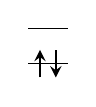
\begin{tikzpicture}[baseline={([yshift=-.5ex]current bounding box.center)},vertex/.style={anchor=base, minimum size=18pt, inner sep=2pt}]
    \draw (0,0.275) -- (0.5,0.275);
    \draw (0,0.725) -- (0.5,0.725);
    \draw[thick,->,>=stealth] (0.15,0.1) -- (0.15,0.45);
    \draw[thick,<-,>=stealth] (0.35,0.1) -- (0.35,0.45);
  \end{tikzpicture}\\[6pt]
  \ket{\Phi_2} = \ket{\psi_{\mathrm{g}}\psi_{\bar{\mathrm{u}}}} 
=
  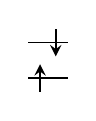
\begin{tikzpicture}[baseline={([yshift=-.5ex]current bounding box.center)},vertex/.style={anchor=base, minimum size=18pt, inner sep=2pt}]
    \draw (0,0.275) -- (0.5,0.275);
    \draw (0,0.725) -- (0.5,0.725);
    \draw[thick,->,>=stealth] (0.15,0.1) -- (0.15,0.45);
    \draw[thick,<-,>=stealth] (0.35,0.55) -- (0.35,0.9);
  \end{tikzpicture}\\[6pt]
  \ket{\Phi_3} = \ket{\psi_{\mathrm{u}}\psi_{\bar{\mathrm{g}}}} 
=
  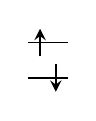
\begin{tikzpicture}[baseline={([yshift=-.5ex]current bounding box.center)},vertex/.style={anchor=base, minimum size=18pt, inner sep=2pt}]
    \draw (0,0.275) -- (0.5,0.275);
    \draw (0,0.725) -- (0.5,0.725);
    \draw[thick,<-,>=stealth] (0.35,0.1) -- (0.35,0.45);
    \draw[thick,->,>=stealth] (0.15,0.55) -- (0.15,0.9);
  \end{tikzpicture}\\[6pt]
    \ket{\Phi_4} = \ket{\psi_{\mathrm{u}}\psi_{\bar{\mathrm{u}}}} 
=
  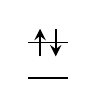
\begin{tikzpicture}[baseline={([yshift=-.5ex]current bounding box.center)},vertex/.style={anchor=base, minimum size=18pt, inner sep=2pt}]
    \draw (0,0.275) -- (0.5,0.275);
    \draw (0,0.725) -- (0.5,0.725);
    \draw[thick,<-,>=stealth] (0.35,0.55) -- (0.35,0.9);
    \draw[thick,->,>=stealth] (0.15,0.55) -- (0.15,0.9);
  \end{tikzpicture}\\[6pt]
      \ket{\Phi_5} = \ket{\psi_{\mathrm{g}}\psi_{\mathrm{u}}} 
=
  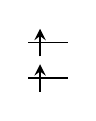
\begin{tikzpicture}[baseline={([yshift=-.5ex]current bounding box.center)},vertex/.style={anchor=base, minimum size=18pt, inner sep=2pt}]
    \draw (0,0.275) -- (0.5,0.275);
    \draw (0,0.725) -- (0.5,0.725);
    \draw[thick,->,>=stealth] (0.15,0.1) -- (0.15,0.45);
    \draw[thick,->,>=stealth] (0.15,0.55) -- (0.15,0.9);
  \end{tikzpicture}\\[6pt]
        \ket{\Phi_6} = \ket{\psi_{\bar{\mathrm{g}}}\psi_{\bar{\mathrm{u}}}} 
=
  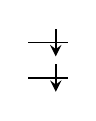
\begin{tikzpicture}[baseline={([yshift=-.5ex]current bounding box.center)},vertex/.style={anchor=base, minimum size=18pt, inner sep=2pt}]
    \draw (0,0.275) -- (0.5,0.275);
    \draw (0,0.725) -- (0.5,0.725);
    \draw[thick,<-,>=stealth] (0.35,0.55) -- (0.35,0.9);
    \draw[thick,<-,>=stealth] (0.35,0.1) -- (0.35,0.45);
  \end{tikzpicture}
\end{align}
Symmetry greatly simplifies this problem.\mnote{Recall that when an operator $\hat{O}$ commutes with the Hamiltonian, $[\hat{H},\hat{O}] = 0$, then it is possible to find a set of states that simultaneously diagonalize $\hat{H}$ and $\hat{O}$. For a set of symmetry operations this result implies that the eigensolutions of $\hat{H}$ may be classified according to the irreducible representations.}
The determinants $\ket{\Phi_1}$ and $\ket{\Phi_4}$ are gerade since the product $\psi_{\mathrm{g}}\psi_{\bar{\mathrm{g}}}$ has symmetry equal to g $\times$ g = g.\mnote{Recall that for molecules that possess a center of inversion the following rules apply: g $\times$ g = g, g $\times$ u = u $\times$ g = u, u $\times$ u = g.}
Determinants $\ket{\Phi_2}$, $\ket{\Phi_3}$, $\ket{\Phi_5}$, $\ket{\Phi_6}$ instead are ungerade.
Spin (which is another symmetry) helps.
Determinants 1--4 have all $M_S = 0$, while 5 and 6 have $M_S = +1$ and $-1$, respectively.
Determinants with different symmetry and spin will not contribute to the same eigenfunction.
As a consequence, the eigenfunctions for H$_2$ will be either a gerade state with $M_S = 0$ and wave function:
\begin{equation}
C_1 \ket{\Phi_1} + C_4 \ket{\Phi_4},
\end{equation}
or a ungerade state with $M_S = 0$ and wave function:
\begin{equation}
C_2 \ket{\Phi_2} + C_3 \ket{\Phi_3},
\end{equation}
or one of the two ungerade states with $M_S = \pm1$ ($\ket{\Phi_5}$, $\ket{\Phi_6}$).

Let us now analyze these determinants in terms of the atomic basis functions.
Consider $\Phi_1$, the lowest energy determinant.
If we plug in the definitions of the spin orbitals we obtain:
\begin{equation}
\begin{split}
\ket{\Phi_1} &= \ket{\psi_{\mathrm{g}} \psi_{\bar{\mathrm{g}}}} = N_{\mathrm{g}}^2 \ket{ (\chi_{1\rm s}^{\rm A} + \chi_{1\rm s}^{\rm B}) \alpha  (\chi_{1\rm s}^{\rm A} + \chi_{1\rm s}^{\rm B}) \beta} \\
&= N_{\mathrm{g}}^2 [ \ket{\chi_{1\rm s}^{\rm A}\alpha \chi_{1\rm s}^{\rm A}\beta}
+ \ket{\chi_{1\rm s}^{\rm A}\alpha \chi_{1\rm s}^{\rm B}\beta}
+ \ket{\chi_{1\rm s}^{\rm B}\alpha \chi_{1\rm s}^{\rm A}\beta} 
+\ket{\chi_{1\rm s}^{\rm B}\alpha \chi_{1\rm s}^{\rm B}\beta}].
\end{split}
\end{equation}
The first and last terms correspond to ionic configurations of electrons: 
\begin{equation}
 \ket{\chi_{1\rm s}^{\rm A}\alpha \chi_{1\rm s}^{\rm A}\beta} \equiv 
 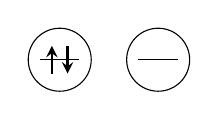
\begin{tikzpicture}[baseline={([yshift=-.5ex]current bounding box.center)},vertex/.style={anchor=base, minimum size=18pt, inner sep=2pt}]
    \draw (0.25,0.5) circle (0.4);
    \draw (0,0.5) -- (0.5,0.5);
    \draw[thick,->,>=stealth] (0.15,0.325) -- (0.15,0.675);
    \draw[thick,<-,>=stealth] (0.35,0.325) -- (0.35,0.675);    
    \draw (1.5,0.5) circle (0.4);
    \draw (1.25,0.5) -- (1.75,0.5);
  \end{tikzpicture}
\end{equation}
and
\begin{equation}
 \ket{\chi_{1\rm s}^{\rm B}\alpha \chi_{1\rm s}^{\rm B}\beta} \equiv 
 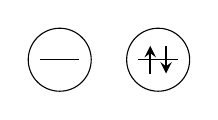
\begin{tikzpicture}[baseline={([yshift=-.5ex]current bounding box.center)},vertex/.style={anchor=base, minimum size=18pt, inner sep=2pt}]
    \draw (0.25,0.5) circle (0.4);
    \draw (0,0.5) -- (0.5,0.5);
    \draw[thick,->,>=stealth] (1.4,0.325) -- (1.4,0.675);
    \draw (1.5,0.5) circle (0.4);
    \draw (1.25,0.5) -- (1.75,0.5);
    \draw[thick,<-,>=stealth] (1.6,0.325) -- (1.6,0.675);
  \end{tikzpicture}
\end{equation}
since both electrons occupy the atomic orbitals on atom A or B.
The remaining contributions describe covalent bonds in which each atomic orbital is occupied with one electrons. These are:
\begin{equation}
 \ket{\chi_{1\rm s}^{\rm A}\alpha \chi_{1\rm s}^{\rm B}\beta} \equiv 
 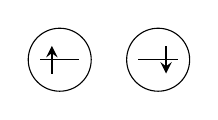
\begin{tikzpicture}[baseline={([yshift=-.5ex]current bounding box.center)},vertex/.style={anchor=base, minimum size=18pt, inner sep=2pt}]
    \draw (0.25,0.5) circle (0.4);
    \draw (0,0.5) -- (0.5,0.5);
    \draw[thick,->,>=stealth] (0.15,0.325) -- (0.15,0.675);
    \draw[thick,<-,>=stealth] (1.6,0.325) -- (1.6,0.675);
    \draw (1.5,0.5) circle (0.4);
    \draw (1.25,0.5) -- (1.75,0.5);
  \end{tikzpicture}
\end{equation}
and
\begin{equation}
 \ket{\chi_{1\rm s}^{\rm B}\alpha \chi_{1\rm s}^{\rm A}\beta} \equiv 
 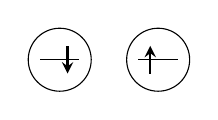
\begin{tikzpicture}[baseline={([yshift=-.5ex]current bounding box.center)},vertex/.style={anchor=base, minimum size=18pt, inner sep=2pt}]
    \draw (0.25,0.5) circle (0.4);
    \draw (0,0.5) -- (0.5,0.5);
    \draw[thick,<-,>=stealth] (0.35,0.325) -- (0.35,0.675);    
    \draw[thick,->,>=stealth] (1.4,0.325) -- (1.4,0.675);
    \draw (1.5,0.5) circle (0.4);
    \draw (1.25,0.5) -- (1.75,0.5);
  \end{tikzpicture}
\end{equation}
All these four determinants contribute equally, so the determinant $\Phi_1$ represents a state that has mixture of 50\% covalent and 50\% ionic electronic configurations.
The determinant $\Phi_4$ is also a 50/50 combination of covalent and ionic terms, but the sign of the covalent contributions is different:
\begin{equation}
\begin{split}
\ket{\Phi_4} &= \ket{\psi_{\mathrm{u}} \psi_{\bar{\mathrm{u}}}} = N_{\mathrm{u}}^2 \ket{ (\chi_{1\rm s}^{\rm A} - \chi_{1\rm s}^{\rm B}) \alpha  (\chi_{1\rm s}^{\rm A} - \chi_{1\rm s}^{\rm B}) \beta} \\
&= N_{\mathrm{u}}^2 [ \ket{\chi_{1\rm s}^{\rm A}\alpha \chi_{1\rm s}^{\rm A}\beta}
- \ket{\chi_{1\rm s}^{\rm A}\alpha \chi_{1\rm s}^{\rm B}\beta}
- \ket{\chi_{1\rm s}^{\rm B}\alpha \chi_{1\rm s}^{\rm A}\beta} 
+\ket{\chi_{1\rm s}^{\rm B}\alpha \chi_{1\rm s}^{\rm B}\beta}].
\end{split}
\end{equation}
Any linear combination of $\Phi_1$ and $\Phi_4$ may be used to represent covalent or ionic states because by carefully choosing $C_1$ and $C_4$ it is possible to cancel the ionic or covalent contributions.

The determinant $\Phi_5$ has $M_S = +1$ and is a component of a triplet state ($S = 1$).
Expanding $\Phi_5$ in terms of spin orbital we find:
\begin{equation}
\begin{split}
\ket{\Phi_5} &= \ket{\psi_{\mathrm{g}} \psi_{\mathrm{u}}} = N_{\mathrm{g}} N_{\mathrm{u}} \ket{ (\chi_{1\rm s}^{\rm A} + \chi_{1\rm s}^{\rm B}) \alpha  (\chi_{1\rm s}^{\rm A} - \chi_{1\rm s}^{\rm B}) \alpha} \\
&= N_{\mathrm{g}} N_{\mathrm{u}}  [
\underbrace{\ket{\chi_{1\rm s}^{\rm A}\alpha \chi_{1\rm s}^{\rm A}\alpha}}_{= 0}
- \ket{\chi_{1\rm s}^{\rm A}\alpha \chi_{1\rm s}^{\rm B}\alpha}
+ \ket{\chi_{1\rm s}^{\rm B}\alpha \chi_{1\rm s}^{\rm A}\alpha} 
- \underbrace{\ket{\chi_{1\rm s}^{\rm B}\alpha \chi_{1\rm s}^{\rm B}\alpha}}_{= 0}] \\
&= 2 N_{\mathrm{g}} N_{\mathrm{u}}  \ket{\chi_{1\rm s}^{\rm B}\alpha \chi_{1\rm s}^{\rm A}\alpha} .
\end{split}
\end{equation}
Where in the last step we used the antisymmetry property of Slater determinants and swapped the two spin orbitals
\begin{equation}
\ket{\chi_{1\rm s}^{\rm A}\alpha \chi_{1\rm s}^{\rm B}\alpha} = -\ket{\chi_{1\rm s}^{\rm B}\alpha \chi_{1\rm s}^{\rm A}\alpha}.
\end{equation}
We also eliminated the Pauli-principle violating terms like this:
\begin{equation}
 \ket{\chi_{1\rm s}^{\rm A}\alpha \chi_{1\rm s}^{\rm A}\alpha} \equiv 
 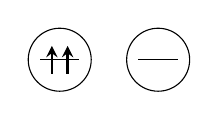
\begin{tikzpicture}[baseline={([yshift=-.5ex]current bounding box.center)},vertex/.style={anchor=base, minimum size=18pt, inner sep=2pt}]
    \draw (0.25,0.5) circle (0.4);
    \draw (0,0.5) -- (0.5,0.5);
    \draw[thick,->,>=stealth] (0.15,0.325) -- (0.15,0.675);
    \draw[thick,->,>=stealth] (0.35,0.325) -- (0.35,0.675);    
    \draw (1.5,0.5) circle (0.4);
    \draw (1.25,0.5) -- (1.75,0.5);
  \end{tikzpicture}
\end{equation}
In other words, this determinant accounts for Fermi correlation.
The state $\Phi_5$ corresponds to having each atomic orbital occupied by one alpha electron.

Finally, we will consider the spin of the determinants.
Apply the operator $\hat{S}^2$ to determinant $\Phi_5$:
\begin{equation}
\begin{split}
\hat{S}^2 \ket{\Phi_5} &= \hat{S}^2  \ket{\psi_{\mathrm{g}} \psi_{\mathrm{u}}} 
= (\hat{S}_{+} \hat{S}_{-}  + \hat{S}_{z}^2 - \hat{S}_{z}) \ket{\psi_{\mathrm{g}} \psi_{\mathrm{u}}}.
\end{split}
\end{equation}
Let us consider these terms in detail\mnote{$\hat{S}_{-}=\hat{s}_{-}(1) + \hat{s}_{-}(2)$.}
\begin{equation}
\hat{S}_{+} \hat{S}_{-} \ket{\psi_{\mathrm{g}} \psi_{\mathrm{u}}}
= \hat{S}_{+} (\ket{\psi_{\bar{\mathrm{g}}} \psi_{\mathrm{u}}} + \ket{\psi_{\mathrm{g}} \psi_{\bar{\mathrm{u}}}}
)
= 2 \ket{\psi_{\mathrm{g}} \psi_{\mathrm{u}}}.
\end{equation}
\begin{equation}
\hat{S}_{z} \ket{\psi_{\mathrm{g}} \psi_{\mathrm{u}}} = \left(\frac{1}{2} + \frac{1}{2}\right) \ket{\psi_{\mathrm{g}} \psi_{\mathrm{u}}} = \ket{\psi_{\mathrm{g}} \psi_{\mathrm{u}}}.
\end{equation}
Putting all together we get
\begin{equation}
\begin{split}
\hat{S}^2 \ket{\Phi_5} &= (\hat{S}_{+} \hat{S}_{-}  + \hat{S}_{z}^2 - \hat{S}_{z}) \ket{\psi_{\mathrm{g}} \psi_{\mathrm{u}}} \\
&= 2 \ket{\psi_{\mathrm{g}} \psi_{\mathrm{u}}} + \ket{\psi_{\mathrm{g}} \psi_{\mathrm{u}}} - \ket{\psi_{\mathrm{g}} \psi_{\mathrm{u}}} = 2 \ket{\psi_{\mathrm{g}} \psi_{\mathrm{u}}}.
\end{split}
\end{equation}
This result shows that $\Phi_5$ is an eigenfunction of $\hat{S}^2$ with eigenvalue equal to 2.
In other words, $S (S + 1) = 2$, which implies $S = 1$.
Therefore, $\Phi_5$ is the component of a triplet state with $M_S = +1$.
Since triplets are triply degenerate, there must be two other components of the triplet.
The $M_S = -1$ component is the determinant $\Phi_6$.

What about the $M_S = 0$ component?  It turns out that this component is contained in determinants $\Phi_2$ and $\Phi_3$.
Let us compute $\hat{S}^2 \ket{\Phi_2}$. We will need the quantity:
\begin{equation}
\begin{split}
\hat{S}_{+} \hat{S}_{-} \ket{\Phi_2}
= \hat{S}_{+} \hat{S}_{-} \ket{\psi_{\mathrm{g}}\psi_{\bar{\mathrm{u}}}}
= \hat{S}_{+} \ket{\psi_{\bar{\mathrm{g}}}\psi_{\bar{\mathrm{u}}}}
= \ket{\psi_{\mathrm{g}}\psi_{\bar{\mathrm{u}}}} + \ket{\psi_{\bar{\mathrm{g}}}\psi_{\mathrm{u}}}
\end{split},
\end{equation}
and
\begin{equation}
\hat{S}_{z} \ket{\psi_{\mathrm{g}}\psi_{\bar{\mathrm{u}}}}
= \left(\frac{1}{2} - \frac{1}{2}\right) \ket{\psi_{\mathrm{g}}\psi_{\bar{\mathrm{u}}}} = 0.
\end{equation}
From these results we find that:
\begin{equation}
\hat{S}^2 \ket{\Phi_2} = \ket{\psi_{\mathrm{g}}\psi_{\bar{\mathrm{u}}}} + \ket{\psi_{\bar{\mathrm{g}}}\psi_{\mathrm{u}}} 
= \ket{\psi_{\mathrm{g}}\psi_{\bar{\mathrm{u}}}} - \ket{\psi_{\mathrm{u}}\psi_{\bar{\mathrm{g}}}} = 
\ket{\Phi_2} - \ket{\Phi_3}.
\end{equation}
This means that $\Phi_2$ is not an eigenfunction of $\hat{S}^2$.
The fact that $\hat{S}^2 \ket{\Phi_2}$ gives back both $\Phi_2$ and $\Phi_3$ is a hint that a \textbf{linear combination} of these two determinants is an eigenfunction of spin.
The following result:
\begin{equation}
\hat{S}^2 \ket{\Phi_3} = \ket{\Phi_2} + \ket{\Phi_3}.
\end{equation}
suggests that we consider the plus and minus combination of $\Phi_2$ and $\Phi_3$:
\begin{equation}
\ket{\Phi_\pm} = \frac{1}{\sqrt{2}} \left(  \ket{\Phi_2} \pm \ket{\Phi_3} \right).
\end{equation}
These two states are such that
\begin{equation}
\hat{S}^2 \ket{\Phi_+} = 0,
\end{equation}
and
\begin{equation}
\hat{S}^2 \ket{\Phi_{-}} = 2 \ket{\Phi_{-}}.
\end{equation}
Therefore, $\Phi_{-}$ is a triplet state while $\Phi_{+}$ is a singlet state.

\end{document}